\documentclass{article}
\usepackage[utf8]{inputenc}
\usepackage{graphics}

\title{HW 4 com org}
\author{Ayush Krishnappa}
\date{October 2022}

\begin{document}

\maketitle

\section{Simplify the following expressions using Boolean algebraic laws. Give each step of your simplification and denote which laws you’re using for each step. Do not skip or combine steps!
}

\begin{itemize}
\large
    \item a) $A \cdot (\overline{A} + B \cdot B) + \overline{(B + A)} \cdot (\overline{A} + B)$\newline
    1. $A \cdot (\overline{A} + B \cdot B) + (\overline{B} \cdot \overline{A}) \cdot (\overline{A} + B)$ DeMorgan's \newline
    2. $A \cdot (\overline{A} + B) + (\overline{B} \cdot \overline{A}) \cdot (\overline{A} + B)$ Idempotent \newline
    3. $(\overline{A} + B) \cdot (A + (\overline{B} \cdot \overline{A}))$ Distributive \newline
    4. $(\overline{A} \cdot A) + (\overline{A} \cdot (\overline{B} \cdot \overline{A})) + (B \cdot A) + (B \cdot (\overline{B} \cdot \overline{A})$ Distributive \newline
    5. $0 + (\overline{A} \cdot \overline{A} \cdot \overline{B}) + (B \cdot A) + (0 \cdot \overline{A})$ Inverse \newline
    6. $(\overline{A} \cdot \overline{B}) + (B \cdot A) + (0 \cdot \overline{A})$ Idempotent \newline
    7. $(\overline{A} \cdot \overline{B}) + (B \cdot A) + 0$ Law of zeroes \newline
    8. Simplified: $(\overline{A} \cdot \overline{B}) + (B \cdot A)$ \newline
    
    \item b) $\overline{C*B} + (A * B * C) + \overline{A + C + \overline{B}}$ \newline
    1. $\overline{C} + \overline{B} + (A * B * C) + \overline{A + C + \overline{B}}$ DeMorgan's \newline
    2. $\overline{C} + \overline{B} + (A * B * C) + \overline{A} * \overline{C} * \overline{\overline{B}}$ DeMorgan's \newline
    3. $\overline{C} + \overline{B} + (A * B * C) + \overline{A} * \overline{C} * B$ double not cancel out \newline
    4. $\overline{C} + \overline{B} + (A * B * C)$ Absorption law $B(AC + \overline{AC})$\newline
    5. $\overline{C} + \overline{B} + (A * B)$ Absorption law $\overline{C} + ABC$\newline
    6. $\overline{C} + \overline{B} + (A)$ Absorption law $\overline{B} + AB$\newline
    7. Simplified: $\overline{C} + \overline{B} + A$ \newline
    
    \item c) $(A + B) * (\overline{A} + C) * (\overline{C} + B)$ \newline
    1. $(A + B) * (\overline{A} * \overline{C} + \overline{A} * B + C * \overline{C} + C * B)$ distributive \newline
    2. $(A + B) * (\overline{A} * \overline{C} + \overline{A} * B + 0 + C * B)$ inverse \newline
    3. $(A * \overline{A} * \overline{C}) + (\overline{A} * B * A) + (C * B * A) + (\overline{A} * \overline{C} * B) + (\overline{A} * B * B) + (C * B * B)$ distributive \newline
    4. $(0 * \overline{C}) + (0 * B) + (C * B * A) + (\overline{A} * \overline{C} * B) + (\overline{A} * B * B) + (C * B * B)$ inverse \newline
    5. $0 + 0 + (C * B * A) + (\overline{A} * \overline{C} * B) + (\overline{A} * B * B) + (C * B * B)$ law of zeroes \newline
    6. $(C * B * A) + (\overline{A} * \overline{C} * B) + (\overline{A} * B) + (C * B)$ Idempotent \newline
    7. $(A * B * C) + (\overline{A} * B) + (C * B)$ Absorption law \newline
    8. Simplified form: $\overline{A} * B + C * B$ Absorption law \newline
    
\end{itemize}

\section{Find all solutions of the following Boolean equations without using the truth tables:}

\begin{itemize}
\large
    \item a) $(\overline{A} + C) * (\overline{B} + D + A) * (D + A * \overline{C}) * (\overline{D} + A) = 1$ \newline
    1. $(D + A + \overline{C})(\overline{D} + A)(\overline{A} * \overline{B}) + (D + A + \overline{C})(\overline{D} + A)(\overline{A} * D) + (D + A + \overline{C})(\overline{D} + A)(\overline{A} * \overline{A}) +
    (\overline{B} + D + A)(D + A + \overline{C})(\overline{D} + A)*C$ Distribution \newline
    2.  $(D + A + \overline{C})(\overline{D} + A)(\overline{A} * \overline{B}) + (D + A + \overline{C})(\overline{D} + A)(\overline{A} * D) + 0 +
    (\overline{B} + D + A)(D + A + \overline{C})(\overline{D} + A)*C$ Inverse \newline
    3. $(\overline{D} + A)(\overline{A} * \overline{B} * D) + 
    (\overline{D} + A)(\overline{A} * \overline{B} * A) + 
    (\overline{D} + A)(\overline{A} * \overline{B} * \overline{C}) + 
    (D + A + \overline{C})(\overline{D} + A)(\overline{A} * \overline{D}) + 
    (\overline{B} + D + A)(D + A + \overline{C})(\overline{D} + A)(C)$ Distribution\newline
    4. $(\overline{D} + A)(\overline{A} * \overline{B} * D) + 
    0 + 
    (\overline{D} + A)(\overline{A} * \overline{B} * \overline{C}) + 
    (D + A + \overline{C})(\overline{D} + A)(\overline{A} * \overline{D}) + 
    (\overline{B} + D + A)(D + A + \overline{C})(\overline{D} + A)(C)$ Inverse\newline
    5. $(\overline{A} * \overline{B} * D * \overline{D}) + 
    (\overline{A} * \overline{B} * D * A) +
    (\overline{D} + A)(\overline{A} * \overline{B} * \overline{C}) +
    (D + A + \overline{C})(\overline{D} + A)(\overline{A} * D) +
    (\overline{B} + D + A)(D + A + \overline{C})(\overline{D} + A)(C)$ Distribution \newline
    6. $0 + 
    0 +
    (\overline{D} + A)(\overline{A} * \overline{B} * \overline{C}) +
    (D + A + \overline{C})(\overline{D} + A)(\overline{A} * D) +
    (\overline{B} + D + A)(D + A + \overline{C})(\overline{D} + A)(C)$ Inverse \newline
    7. $(\overline{A} * \overline{B} * \overline{C} * \overline{D}) +
    (\overline{A} * \overline{B} * \overline{C} * A) +
    (D + A + \overline{C})(\overline{D} + A)(\overline{A} * D) +
    (\overline{B} + D + A)(D + A + \overline{C})(\overline{D} + A)(C)$ Distribution \newline
    8. $(\overline{A} * \overline{B} * \overline{C} * \overline{D}) +
    0 +
    (D + A + \overline{C})(\overline{D} + A)(\overline{A} * D) +
    (\overline{B} + D + A)(D + A + \overline{C})(\overline{D} + A)(C)$ Inverse \newline
    9. $(\overline{A} * \overline{B} * \overline{C} * \overline{D}) +
    (C * \overline{B} * A) + (\overline{D} + A)(C * D * D) + (\overline{D} + A)(C * D * A) + (\overline{D} + A)(C * D * \overline{C}) + (D + A + \overline{C})(\overline{D} + A)(C * A)$ Distribution \newline
    10. $(\overline{A} * \overline{B} * \overline{C} * \overline{D}) +
    (C * \overline{B} * A) + (\overline{D} + A)(C * D) + (\overline{D} + A)(C * D * A) + (\overline{D} + A)(C * D * \overline{C}) + (D + A + \overline{C})(\overline{D} + A)(C * A)$ Idempotent \newline
    11. $(\overline{A} * \overline{B} * \overline{C} * \overline{D}) +
    (C * \overline{B} * A) + (\overline{D} + A)(C * D) + 0 + (\overline{D} + A)(C * D * \overline{C}) + (D + A + \overline{C})(\overline{D} + A)(C * A)$ Inverse \newline
    12. $(\overline{A} * \overline{B} * \overline{C} * \overline{D}) +
    (C * \overline{B} * A) + (\overline{D} + A)(C * D) +
    (D + A + \overline{C})(\overline{D} + A)(C * A)$ Absorption law \newline
    13. $(\overline{A} * \overline{B} * \overline{C} * \overline{D}) +
    (C * \overline{B} * A) + (C * D * A) + (\overline{D} + A)(C * A * D) +
    (\overline{D} + A)(C * A * A) + (\overline{D} + A)(C * A * \overline{C})$ Distribution \newline
    14. $(\overline{A} * \overline{B} * \overline{C} * \overline{D}) +
    (C * \overline{B} * A) + (C * D * A) + (\overline{D} + A)(C * A * D) +
    (\overline{D} + A)(C * A) + (\overline{D} + A)(C * A * \overline{C})$ Idempotent \newline
    15. $(\overline{A} * \overline{B} * \overline{C} * \overline{D}) +
    (C * \overline{B} * A) + (C * D * A) + (\overline{D} + A)(C * A * D) +
    (\overline{D} + A)(C * A) + 0$ Inverse \newline 
    16. $(\overline{A} * \overline{B} * \overline{C} * \overline{D}) +
    (C * \overline{B} * A) + (C * D * A) + (\overline{D} + A)(C * A)$ Absorption \newline
    17. $(\overline{A} * \overline{B} * \overline{C} * \overline{D}) +
    (C * \overline{B} * A) + (C * D * A) + (C * A * \overline{D}) + (C * A * A)$ Distribution \newline
    18. $(\overline{A} * \overline{B} * \overline{C} * \overline{D}) +
    (C * \overline{B} * A) + (C * D * A) + (C * A * \overline{D}) + (C * A)$ Idempotent \newline
    19. $(\overline{A} * \overline{B} * \overline{C} * \overline{D}) + 
    (C * D * A) + (C * A * \overline{D}) + (C * A)$ Absorption law \newline
    20. $(\overline{A} * \overline{B} * \overline{C} * \overline{D}) + 
    (C * A * \overline{D}) + (C * A)$ Absorption law \newline
    21. $(\overline{A} * \overline{B} * \overline{C} * \overline{D}) + 
    (C * A)$ Absorption law \newline
    22. Simplified form: $(\overline{A} * \overline{B} * \overline{C} * \overline{D}) + (C * A)$ \newline
    
    For $(\overline{A} * \overline{B} * \overline{C} * \overline{D}) + 
    (C * A)$ = 1 the different possibilities for A, B, C, and D are \newline
    {A = 0, B = 0, C = 0, D = 0} \newline
    {A = 1, B = 0, C = 1, D = 0} \newline
    {A = 1, B = 0, C = 1, D = 1} \newline
    {A = 1, B = 1, C = 1, D = 0} \newline
    {A = 1, B = 1, C = 1, D = 1} \newline
    
    
    \item b) $(((\overline{K} * L * N) * (L * M)) + ((\overline{K} + L + N) * (K * \overline{L} * M))) * (\overline{K} + \overline{N}) = 1$ \newline
    1. $(\overline{K} + \overline{N}) * \overline{K} * L * N * (L + M) + (\overline{K} + \overline{N}) * (\overline{K} + L + N) * K * \overline{L} * \overline{M} = 1$ Distribution \newline
    2. $\overline{K} * L * N * (L + M) * \overline{K} + \overline{K} * L * N * (L + M) * \overline{N} * (\overline{K} + \overline{N}) * (\overline{K} + L + N) * K * \overline{L} * \overline{M} = 1$ Distribution \newline
    3. $\overline{K} * L * N * (L + M) + \overline{K} * L * N * (L + M) * \overline{N} * (\overline{K} + \overline{N}) * (\overline{K} + L + N) * K * \overline{L} * \overline{M} = 1$ Idempotent \newline 
    4. $\overline{K} * L * N * (L + M) + 0 + (\overline{K} + \overline{N}) * (\overline{K} + L + N) * K * \overline{L} * \overline{M} = 1$ Inverse \newline 
    5. $\overline{K} * L * N * L + \overline{K} * L * N * M + (\overline{K} + \overline{N}) * (\overline{K} + L + N) * K * \overline{L} * \overline{M} = 1$ Distributive \newline
    6. $\overline{K} * L * N + \overline{K} * L * N * M + (\overline{K} + \overline{N}) * (\overline{K} + L + N) * K * \overline{L} * \overline{M} = 1$ Idempotent \newline
    7. $\overline{K} * L * N + (\overline{K} +\overline{N}) * (\overline{K} + L + N) * K * \overline{L} * \overline{M} = 1$ Absorption \newline
    8. $\overline{K} * L * N + (\overline{K} + L + N) * K * \overline{L} * \overline{M} * \overline{K} + (\overline{K} + L + N) * K * \overline{L} * \overline{M} * \overline{N} = 1$ Distribution \newline
    9. $\overline{K} * L * N + 0 + 0 = 1$ Inverse \newline
    10. Simplified: $\overline{K} * L * N = 1$ \newline 
    
    For this expression to be true or 1, the possible values of K, L, M, and N are \newline
    K = {0}, L = {1}, N = {1}, M = {0} \newline
    K = {0}, L = {1}, N = {1}, M = {1} \newline
    The value of M does not matter since its not included in the simplified expression, for the expression !K \& L \& N to be true all 3 components must be true, which is why the two solutions above work. \newline
\end{itemize}

\section{Simplify the following expression by first constructing a truth table, using that truth table to
construct a K-map, and then using that K-map to simplify.} 

\begin{itemize}
\large
    \item $Q = (\overline{X} * \overline{Y} * Z) + (X * Y * \overline{Z}) +
    (\overline{X} + Y + \overline{Z}) + (X + \overline{Y} + \overline{Z})$ \newline
    
  \item
    \begin{tabular}{ccC|c}
      $X$&$Y$&$Z$&$Q$&\\
      \hline 
      \textsc{0}&\textsc{0}&\textsc{0}&\textsc{1}\\
      \textsc{0}&\textsc{0}&\textsc{1}&\textsc{0}\\
      \textsc{0}&\textsc{1}&\textsc{0}&\textsc{1}\\
      \textsc{0}&\textsc{1}&\textsc{1}&\textsc{0}\\
      \textsc{1}&\textsc{0}&\textsc{0}&\textsc{1}\\
      \textsc{1}&\textsc{0}&\textsc{1}&\textsc{0}\\
      \textsc{1}&\textsc{1}&\textsc{0}&\textsc{1}\\
      \textsc{1}&\textsc{1}&\textsc{1}&\textsc{0}\\
    \end{tabular}
    
    K-map \newline
    \resizebox{100mm}{!}{\includegraphics{k-map.png}}\newline
    Simplified expression from k-map: $Q = \overline{Z} $
    
\end{itemize}

\section{Convert the following truth table into its sum of products representation:}

$O = (\overline{A} * \overline{B} * \overline{C}) + (\overline{A} * B * \overline{C}) + (\overline{A} * B * C) + (A * B * C)$

\section{Draw a logical circuit diagram that represents the above sum of products expression using OpenCircuits (https://opencircuits.io/). Clearly label all inputs/outputs and all components. Make sure you connect appropriate input components (e.g., buttons, switches, clocks, etc.) and output components (e.g., LEDs, displays, etc.) to facilitate testing of your circuit.}\newline
\resizebox{200mm}{!}{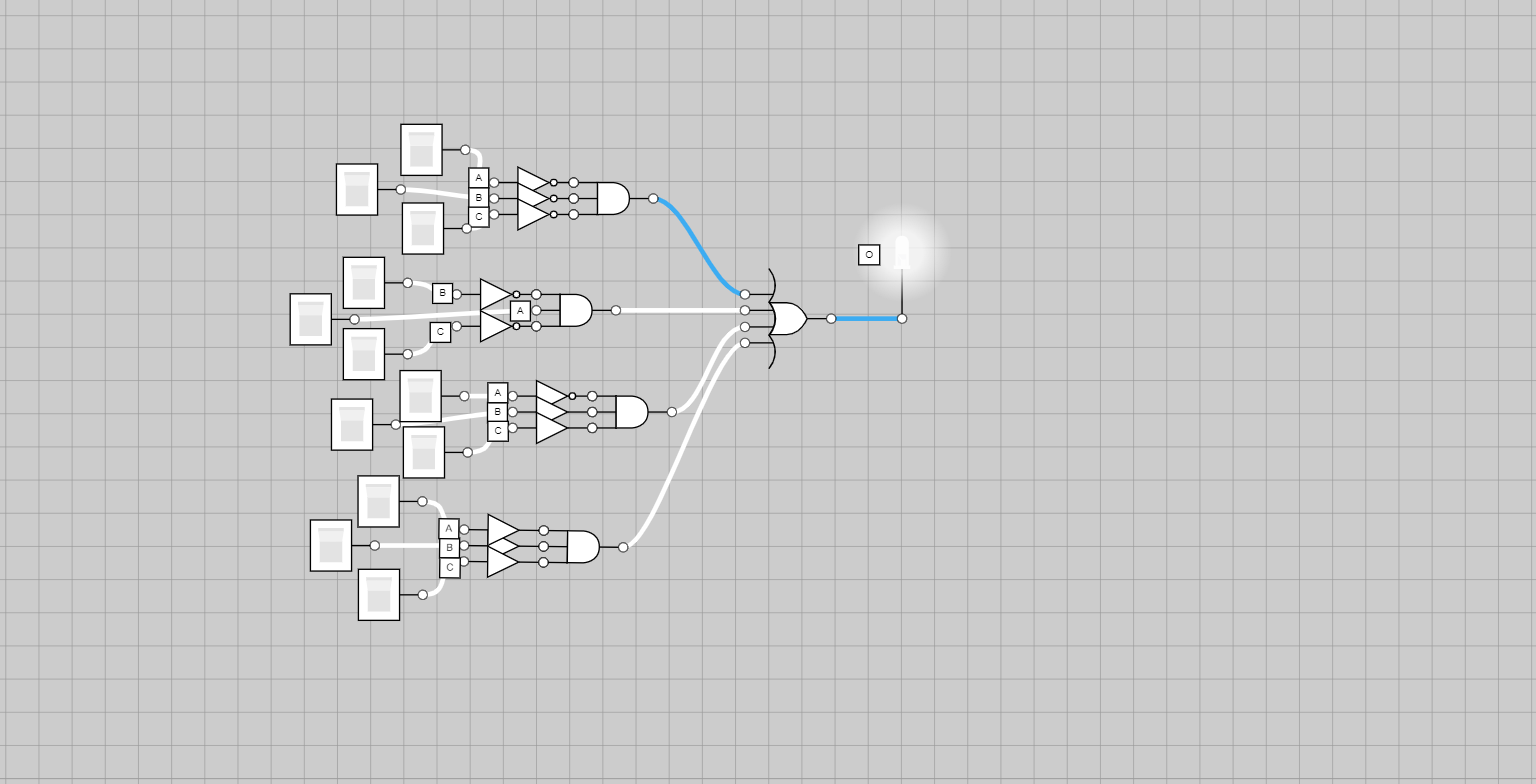
\includegraphics{HW4p5Circuit.png}}\newline


\section{Test you circuit by supplying appropriate inputs and observing the expected values of the
output. Explain why your set of tests is sufficient to prove that your logical circuit does in
fact implement the required Boolean function. For each test, provide a picture (snapshot) of
your circuit. Insert all such pictures in the hw4.pdf PDF file. You can download pictures
(PNG, JPEG, or PDF) of your circuit diagram using OpenCircuits’ “Export Image” feature.}
\large


\begin{itemize}
    \item Test 1, all false inputs for first gate, shows true since first switch equates to true when all inputs are false for A, B, and C (not gates for all inputs)\newline
    \resizebox{200mm}{!}{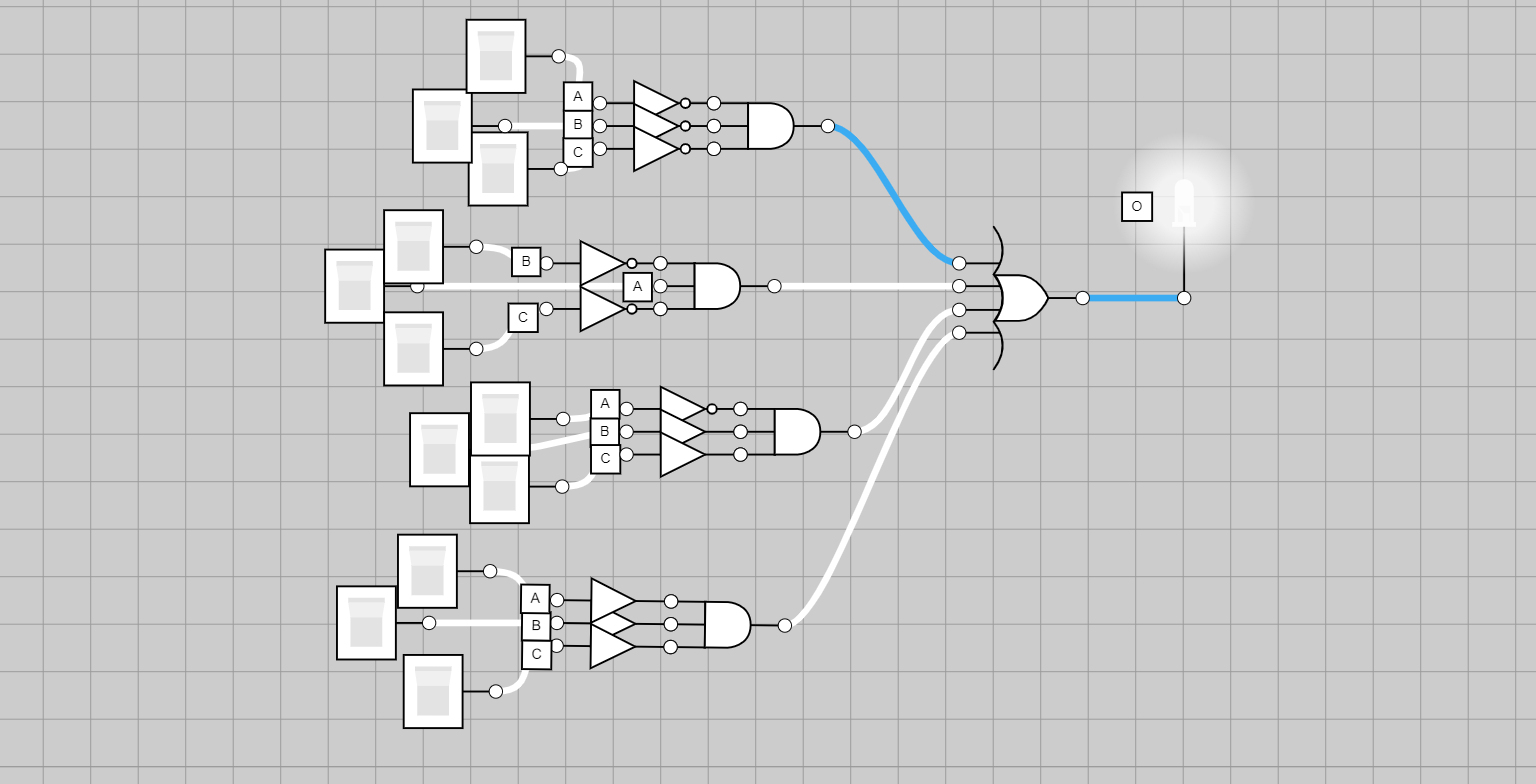
\includegraphics{HW4p5test1.png}}\newline
    
    \item Test 2, true input for B in second gate, and false for A and C, outputs True which matches the truth table\newline
    \resizebox{200mm}{!}{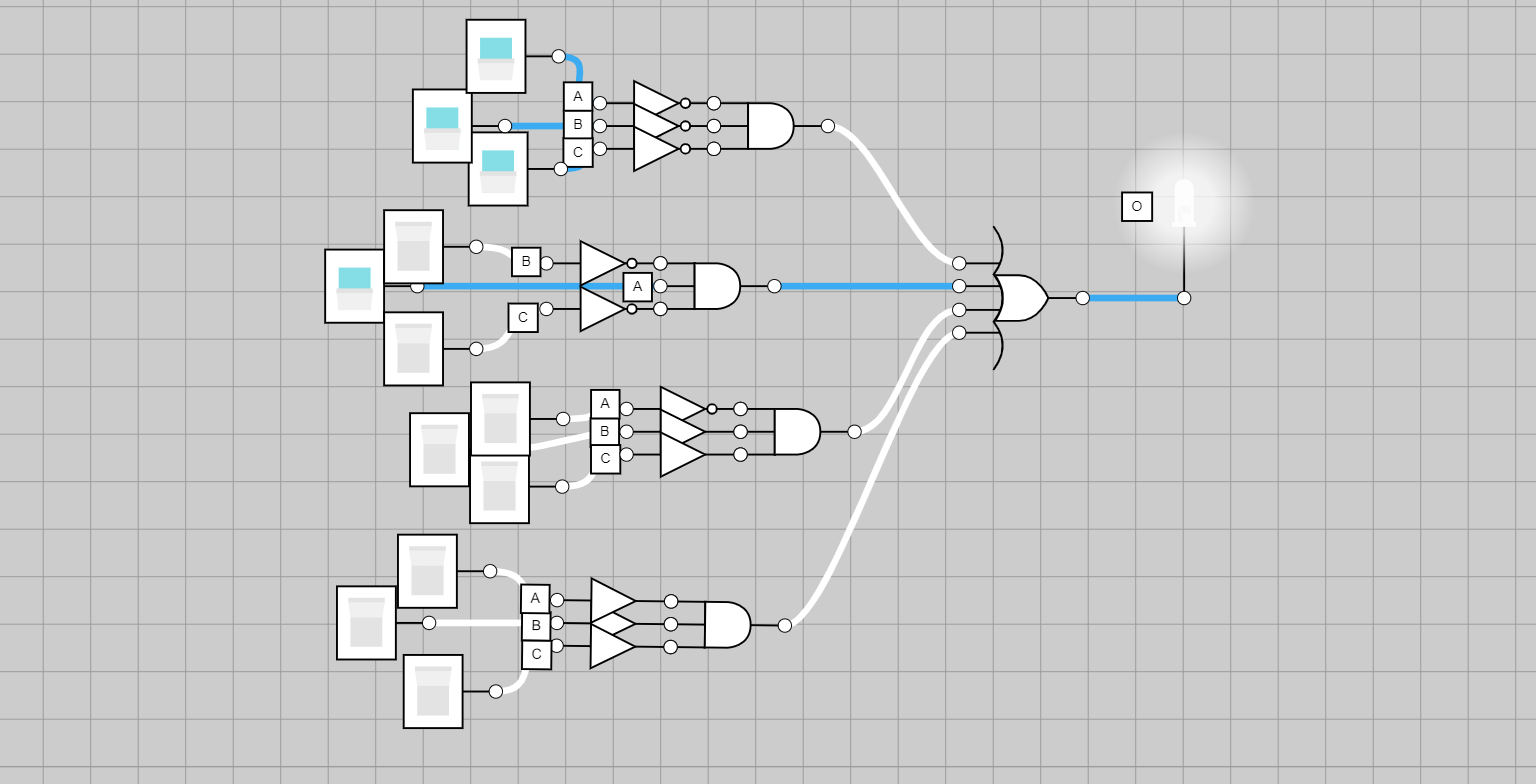
\includegraphics{HW4p5test2.png}}\newline
    
    \item Test 3, True inputs for B and C in gate 3, false input for A, outputs true which matches the truth table \newline
    \resizebox{200mm}{!}{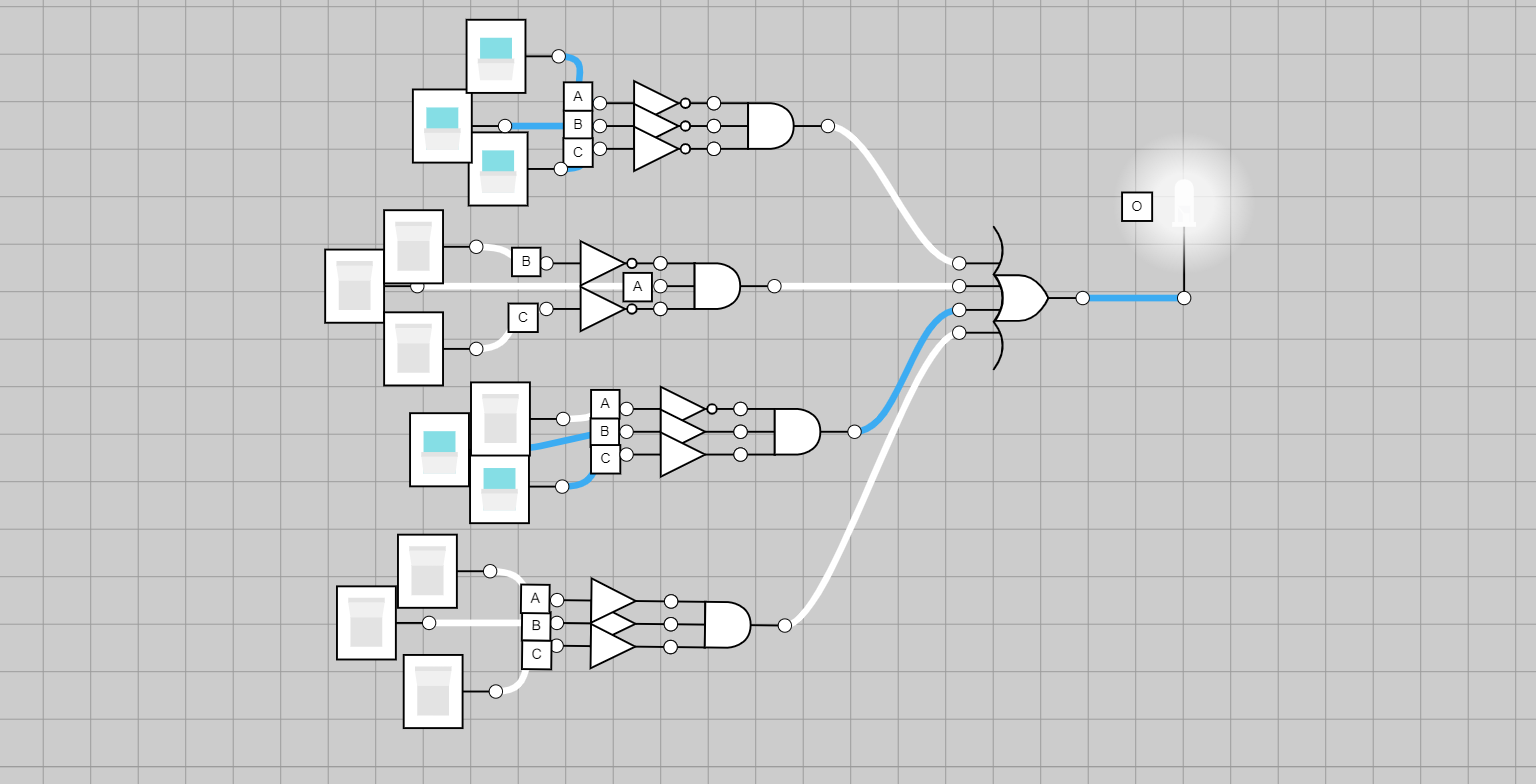
\includegraphics{HW4p5test3.png}}\newline
    
    \item Test 4, True inputs for A, B, and C in gate 4, outputs true which matches truth table \newline
    \resizebox{200mm}{!}{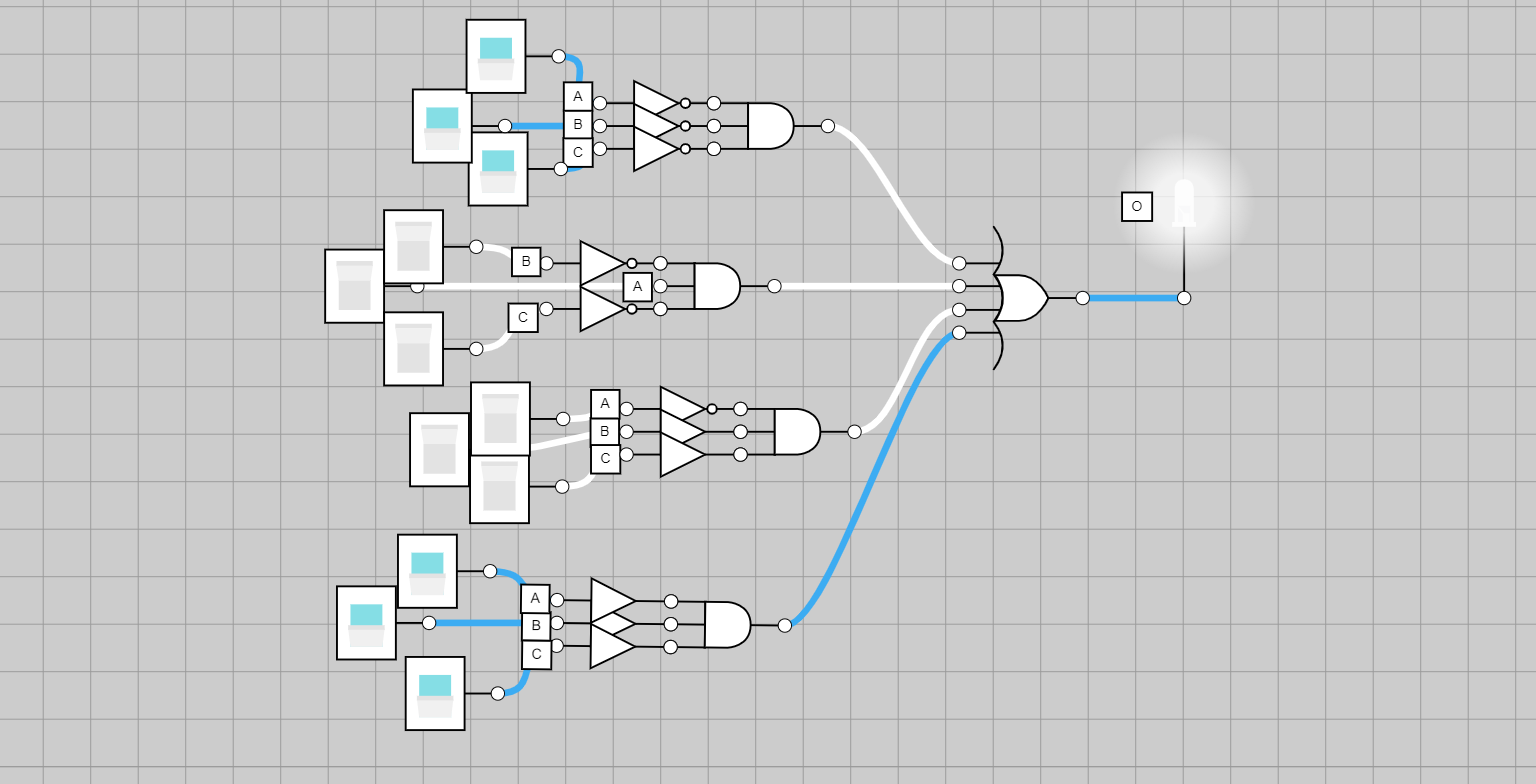
\includegraphics{HW4p5test4.png}}\newline
    
    \item Test 5, All false inputs for all gates, outputs false which matches the false outputs for truth table \newline
    \resizebox{200mm}{!}{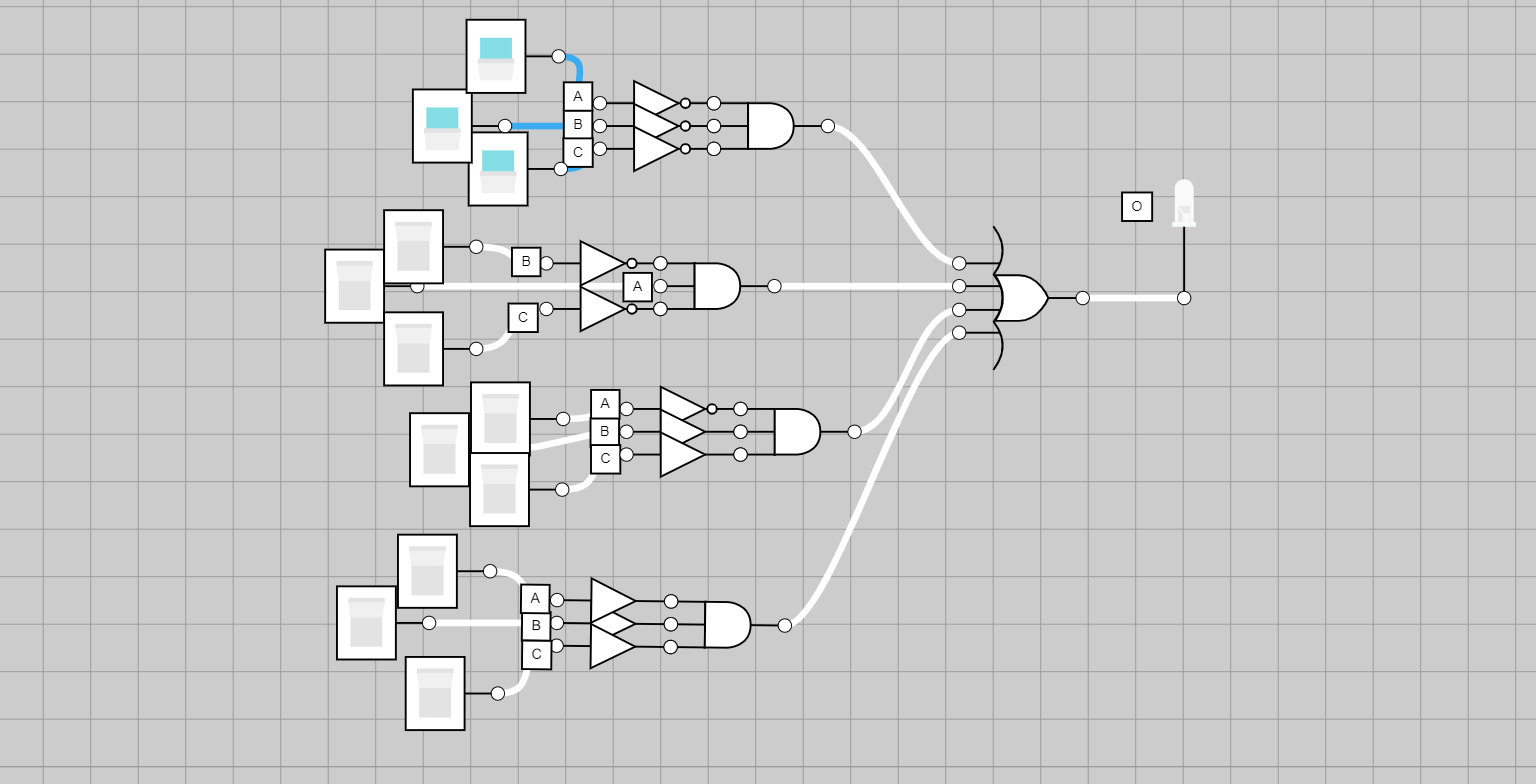
\includegraphics{HW4p5test5.png}}\newline
\end{itemize}

\section{Given inputs A and B, show that NOR $\overline{(A + B)}$ is functionally complete by giving logical
circuits equivalent to AND ${(A * B)}$, OR {(A + B)}, and NOT $\overline{A}$ gates using only NOR
gates in their construction.
}
\large

\begin{itemize}
    \item $(A*B) = NOR(NOR(A+A) + NOR(B+B))$\newline
    \resizebox{200mm}{!}{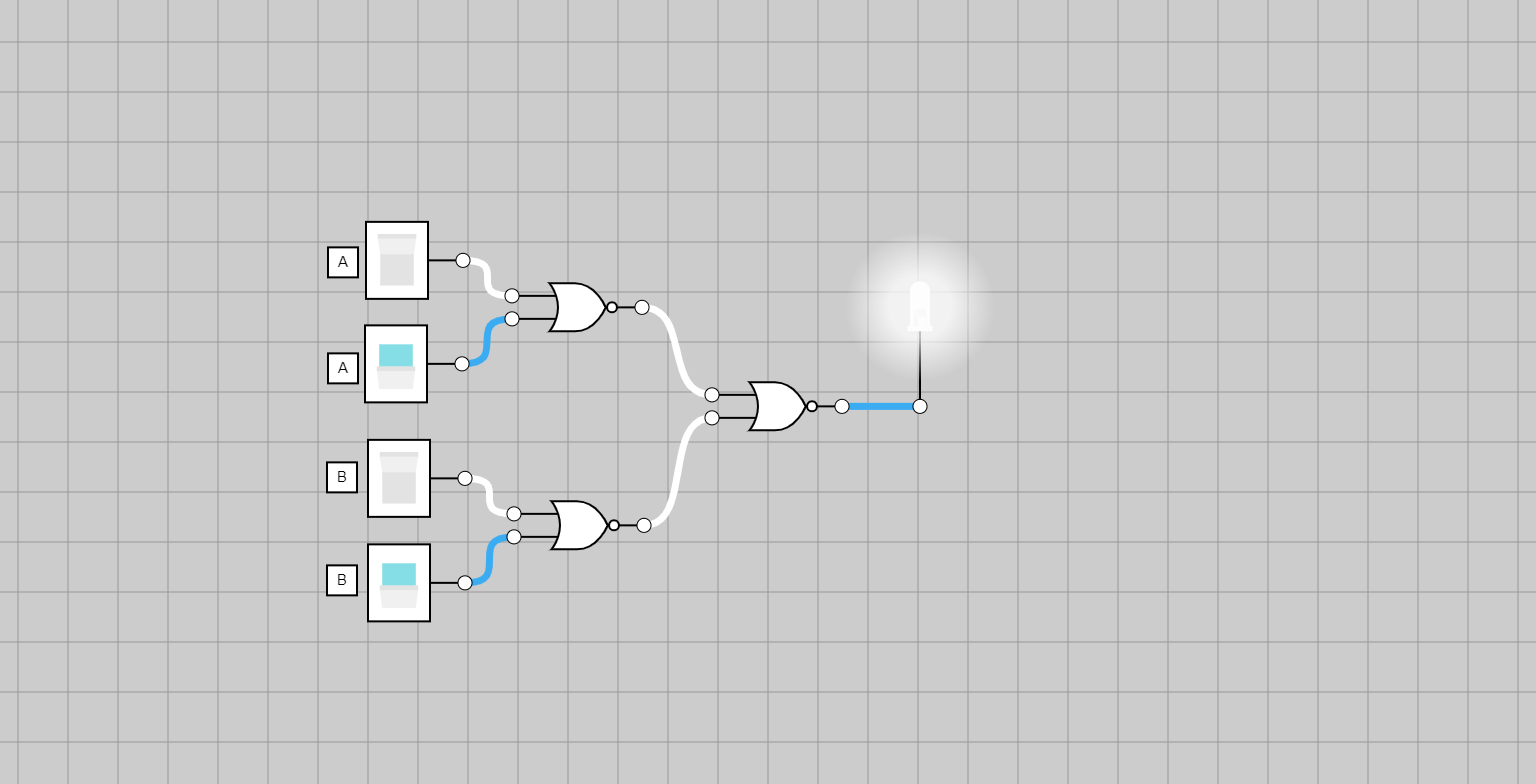
\includegraphics{HW4p7p1.png}}\newline
    As you can see in this image the only time the output is true is when one of the A inputs is true and one of the B inputs is true, otherwise output is always false (equivalent to truth table for (A*B)) \newline
    
    \item $(A+B) = NOR(NOR(A+B) + NOR(A+B))$ \newline
    \resizebox{200mm}{!}{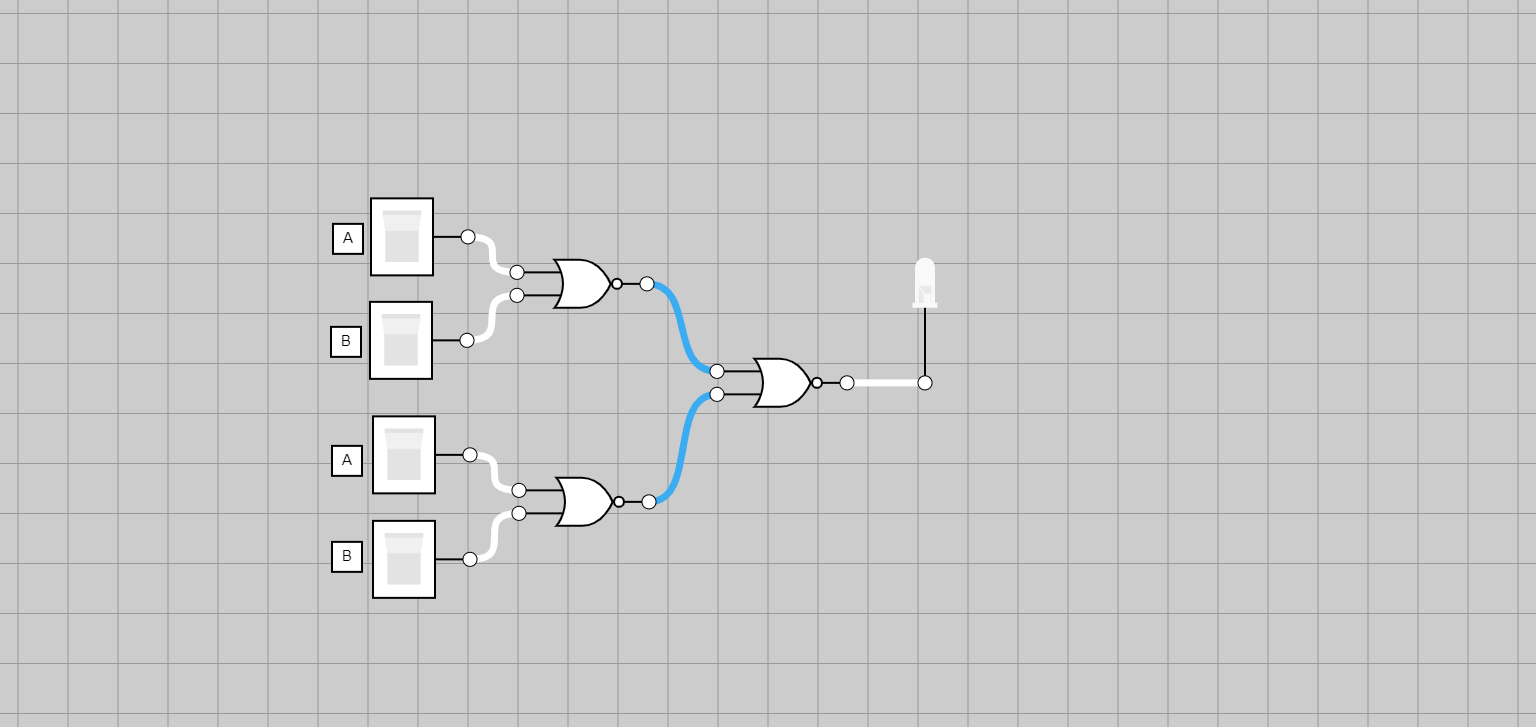
\includegraphics{HW4p7p2.png}}\newline
    For this example the only inputs in the truth table where the output is false, is when both A and B are false, as the image shows when all inputs are false output is false. When either side has one switch turned on the output is true, similar to example above but labels are now switched with one A and B on each side {matches truth table for A OR B using only NOR gates}\newline
    
    \item $NOT(A) = NOR(A + A)$ \newline
    \resizebox{200mm}{!}{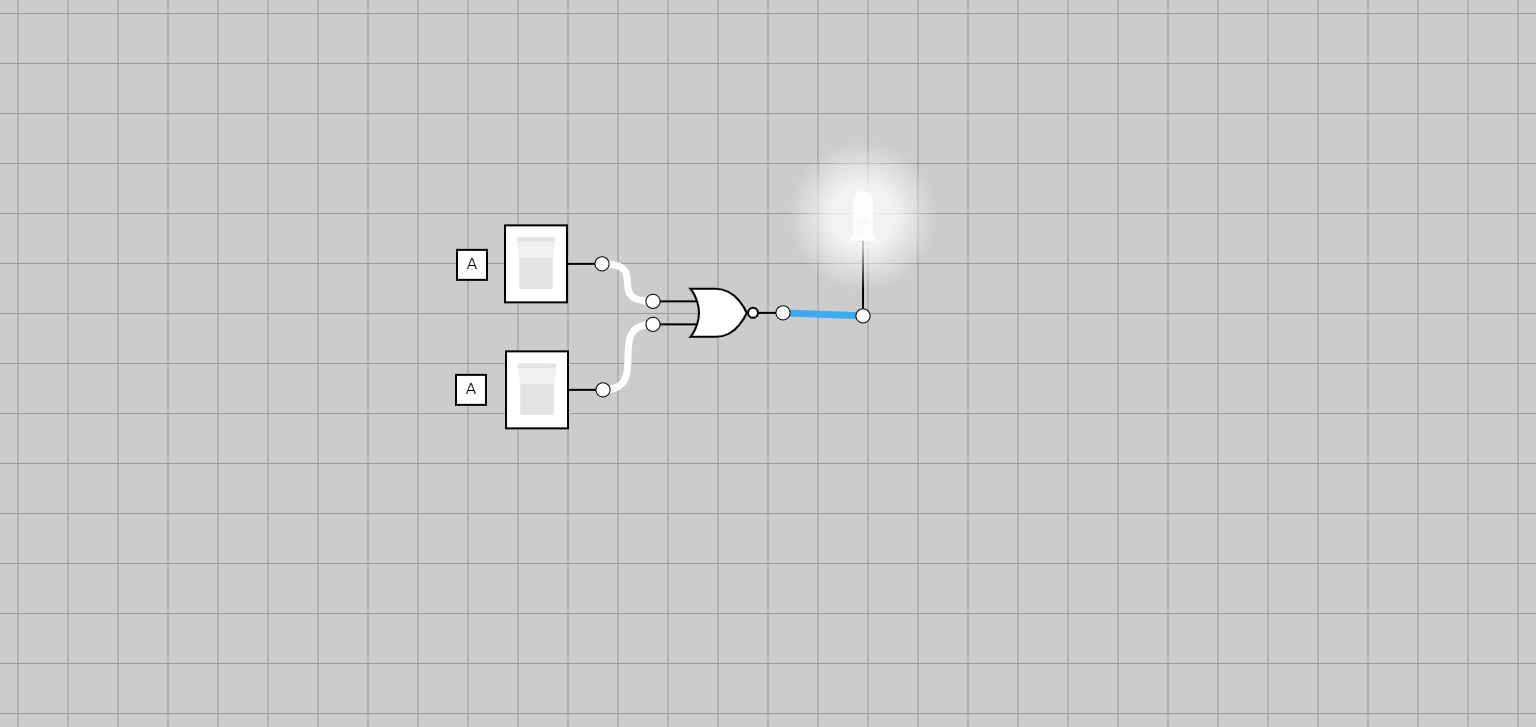
\includegraphics{HW4p7p3.png}}\newline
    AS you can see in the image the output shows true when both inputs are false, when either input is true the output is false, essentially matching the truth table for NOT(A) \newline
    
\end{itemize}

\section{9.13.1}
\large

\begin{itemize}
    \item $(5ED4)_{16}\ = (0101\ 1110\ 1101\ 0100)_2$ \newline
    $(07A4)_{16}\ = (0000\ 0111\ 1010\ 0100)_2$ \newline
    Subtracting the two we get $= (0101\ 0111\ 0011\ 0000)_2$ \newline
    Converting to hexidecimal numbers $= (0101 = 5)\ (0111 = 7)\ (0011 = 3)\ (0000 = 0)\ = (5730)_{16}$ \newline
    $(5ED4)_{16} - (07A4)_{16} = (5730)_{16}$ \newline
\end{itemize}

\section{9.13.2}
\large

\begin{itemize}
    \item $(5ED4)_{16}\ = (0101\ 1110\ 1101\ 0100)_2$ \newline
    $(07A4)_{16}\ = (0000\ 0111\ 1010\ 0100)_2$ \newline
    Both the numbers have a 0 as the Most Significant Bit(leftmost bit) hence they are both positive and subtraction can be carried out normally \newline 
    
    1's compliment of 07A4 = 1111 1000 0101 1011 (inverting the bits, i.e 0 to 1 and 1 to 0) \newline
    
    2's compliment of 07A4 = 1111 1000 0101 1100 (adding 1 to the 1's compliment)\newline
    
    Answer = 0101 1110 1101 0100 + 1111 1000 0101 1100 = 0101 0111 0011 0000 (with a carry of 1) \newline
    
    Hence the result is 0101 0111 0011 0000 or 5730 in hexadecimal \newline
\end{itemize}

\section{9.13.6}
\large

\begin{itemize}
    \item The given numbers 185 and 122 are unsigned 8-bit integers so we don't need to convert them. \newline
    
    Difference: 185 - 122 = 63 \newline
    
    63 in binary is (00111111) \newline
    
    This binary number is represented in 8 bits so their is no underflow or overflow, meaning neither. \newline
\end{itemize}

\section{9.13.10}
\large

\begin{itemize}
    \item Convert first decimal to binary and then take the 2’s complement and Add 1 \newline
    
    A=151=10010111 (binary) \newline
    B=214=11010110 (binary) \newline
    
    A's 2 compliment= 0110 1001 (105) \newline
    B's 2 compliment = 00101010 (42) \newline
    
    subtraction on A-B = 0011 1111 (63) \newline
    
    Since signed 8-bit integers range is -128~127, the result using saturating arithmetic is 63. \newline
    
\end{itemize}

\section{9.13.11}
\large

\begin{itemize}
    \item Convert first decimal to binary and then take the 2’s complement and Add 1 \newline
    
    A=151=10010111 (binary) \newline
    B=214=11010110 (binary) \newline
    
    A's 2 compliment= 0110 1001 (105) \newline
    B's 2 compliment = 00101010 (42) \newline
    
    addition on A+B = 01111111 (127) \newline
    
    Since signed 8-bit integers range is -128~127, the result using saturating arithmetic is 127, not 365. \newline
    
\end{itemize}

\section{9.13.20}
\large

\begin{itemize}
    \item Binary representation of the hexadecimal number (0x0C000000) = $0000\ 1100\ 0000 0000\ 0000\ 0000\ 0000\ 0000_{two}$ \newline
    
    32nd bit is 0, so both two's complement and unsigned integer represent same decimal number. So, for unsigned integer we get $(0*16)^7 + (12*16)^7 + (0*16)^5 + (0*16)^4 + (0*16)^3 + (0*16)^2 + (0*16)^1 + (0*16)^0$ = $0 + 12*16777216 + 0 + 0 + 0 + 0 + 0 + 0 = 2013266529$ \newline
    
    So both the unsigned integer and two's complement are represented as 201326529 as a decimal number. \newline
    
\end{itemize}

\section{9.13.21}
\large

\begin{itemize}
    \item Binary representation of the hexadecimal number (0x0C000000) = $0000\ 1100\ 0000 0000\ 0000\ 0000\ 0000\ 0000_{two}$ \newline
    
    Divided into two sub fields opcode and target\newline
    First 6 bits represent opcode remaining bits represent target\newline
    Bit pattern divided as\newline
    opcode: 000011\newline
    target: 00 0000 0000 0000 0000 0000 0000\newline
    
    opcode represents jal(jump and link instruction)\newline
    Therefore the MIPS instruction Jal is used for the bit pattern 0x0C000000 is placed into the instruction register \newline
    
\end{itemize}

\section{Give a reason why we use two’s complement representation for negative numbers in computer
arithmetic. Give an example of its usage.}
\large

\begin{itemize}
    \item We use two's complement to represent negative numbers in computer arithmetic so that we can use the same logical circuit to perform addition and subtraction. For example to add 6+3 using 5 bit two's complement 
    
    00110 + 00011 = 01001\newline
    Now to subtract we rewrite as 6 + (-3) instead of 6-3 to reuse addition circuit \newline 
    00110 + 11101 = 00011\newline
    
    Looking at this example we can see how much simpler it is made by using the same logical circuit then making a new one to accommodate for both subtraction and addition. 
    
\end{itemize}





\end{document}
